\section{Medotología}


\subsection{Obtención de datos}

La primera parte de la investigación consistió en la identificación y exploración
 de las fuentes de datos disponibles. Se utilizó las
bases de datos eólicas de un proveedor externo (Vaisala Inc) y se trabajó
en una estrategia de muestreo significativa de
480 series de tiempo regularmente espaciados en el departamento de Nariño,
con la cual se espera construir los mapas de potencial eólico
necesarios a 50 y 120 metros de altura. 

Las series de tiempo son conjuntos de reánalisis de datos MERRA (Modern Era Retrospective-analysis for Research and Applications) la cual
tiene una mayor resolucion espacial y temporal (por hora), cada punto contiene
atributos como: latitude, longitud, timestamp, presión, temperatura, velocidad y direccion del viento

\subsection{Procesamiento de datos}

Las series de tiempo fueron procesadas para ser subidas en una base de datos, la figura~\ref{fig:windET} muestra el modelo
entidad relación con las siguientes tablas:

Tabla stations: esta tabla contiene las 480 estaciones con latitud y longitud, de las series de tiempo entregadas por Vaisala Inc.

Tabla timeseries50 y timeseries120: se guardan las series de tiempo desde el año 1980 a 2014 a 50 y 120 metros de altura respectivamente.

Tabla beststations: en esta tabla se guarda las estaciones que con un análisis muestra las mejores 50 estaciones.

Tabla patternbyhourclosed50 y patternbyhourclosed120: en esta tabla se guardaran los patrones detectados en el análisis
de asociación que se mostrará mas adelante con las series de tiempo a 50 y 120 metros de altura.


\begin{figure}
  \centering
  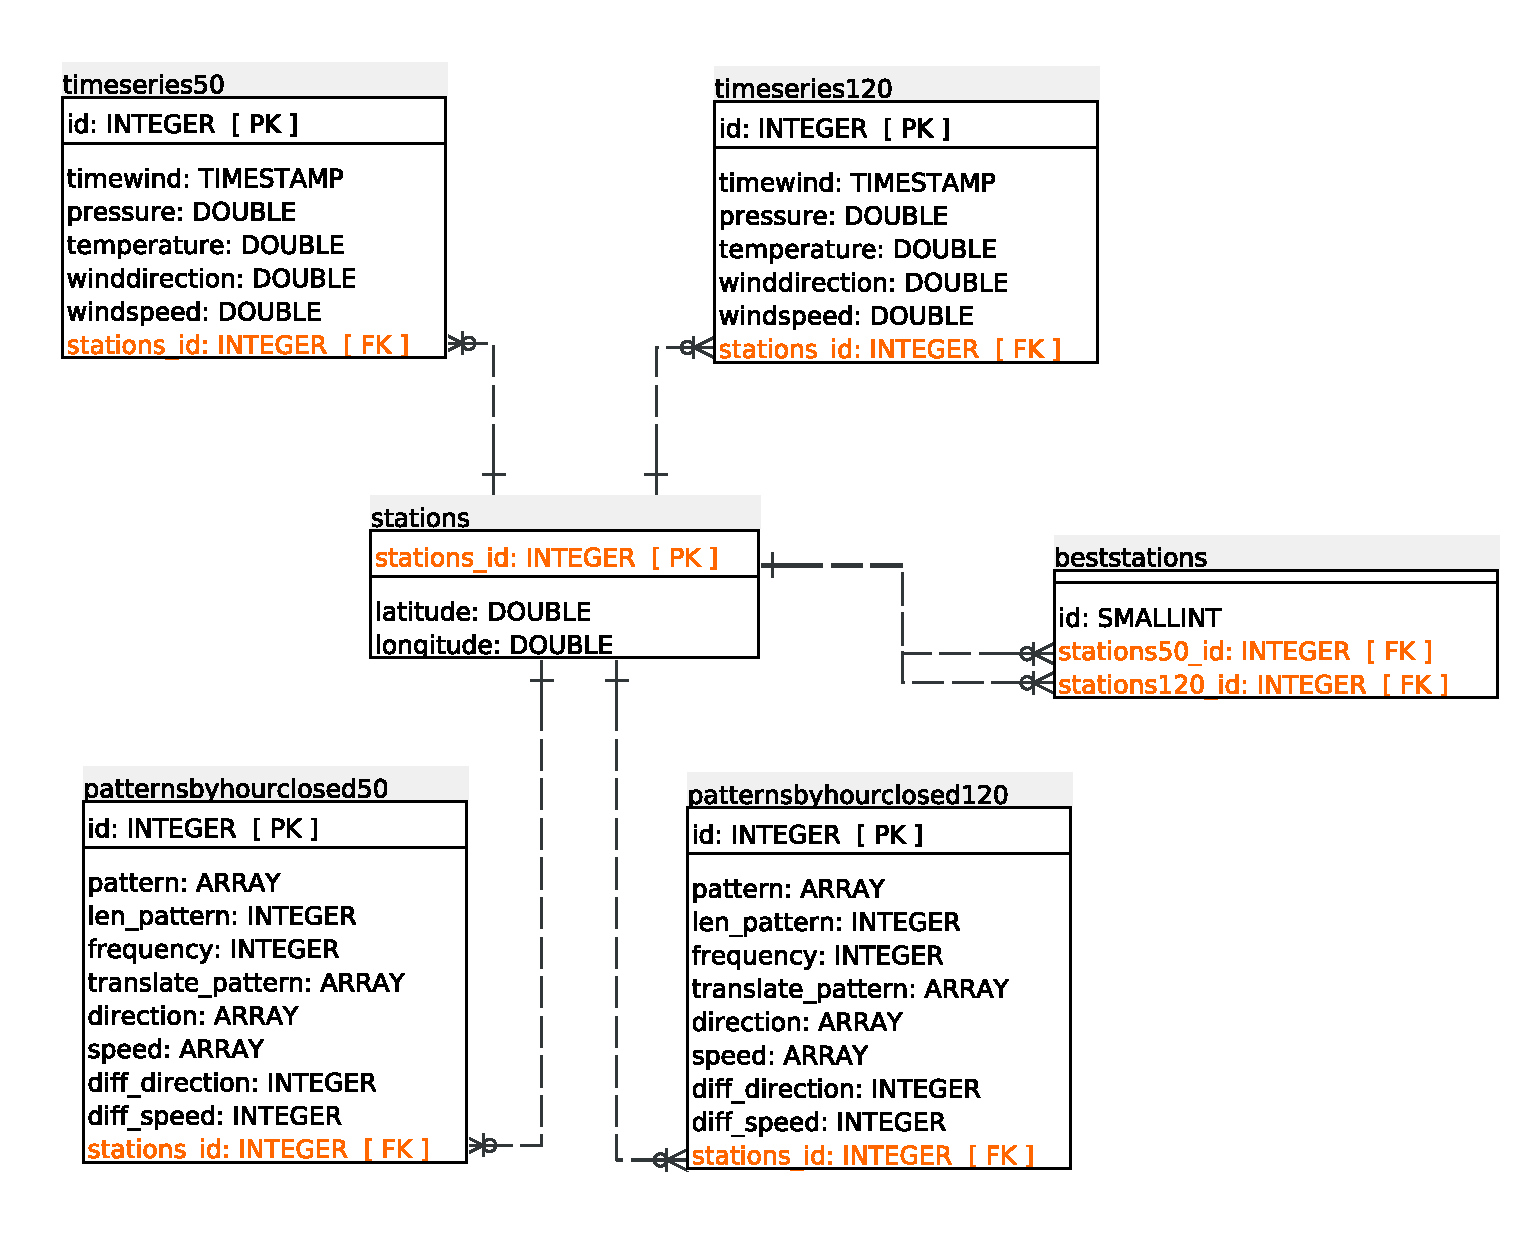
\includegraphics[width = 9cm]{windET.pdf}
  \caption{Modelo entidad relación wind}
  \label{fig:windET}
\end{figure}


%\subsection{Anális exploratorio de datos}

%Aquí se coloca la parte de exploración de datos.


\subsection{Construcción mapas de velocidad de viento}

Para la construcción de mapas de biomasa se utilizó el método Kriging que provee una solución al problema 
de la estimación basada en un modelo continuo de variación espacial estocástica, el objetivo de Kriging es el de estimar el valor de una 
variable aleatoria, Z, en uno o más puntos no muestreados o sobre grandes bloques. 

El método Kriging recibe como entrada datos de la muestra, y una malla dependiendo de la resolución que se quiera obtener, por ello los datos de muestra se
obtuvieron al descomponer la dirección del viento en sus componentes rectangulares multiplicarlas por la velocidad y luego agruparlos en cada punto por mes, año y uno general.
; y la 
 malla se construyó con puntos regulares espaciados cada 450 metros. 
 
 En la figura~\ref{fig:meses}, figura~\ref{fig:anios}, figura~\ref{fig:total}  se muestra los mapas obtenidos por meses, años y general entre el año 2000 a 2014 respectivamente. 

\begin{figure}
  \centering
  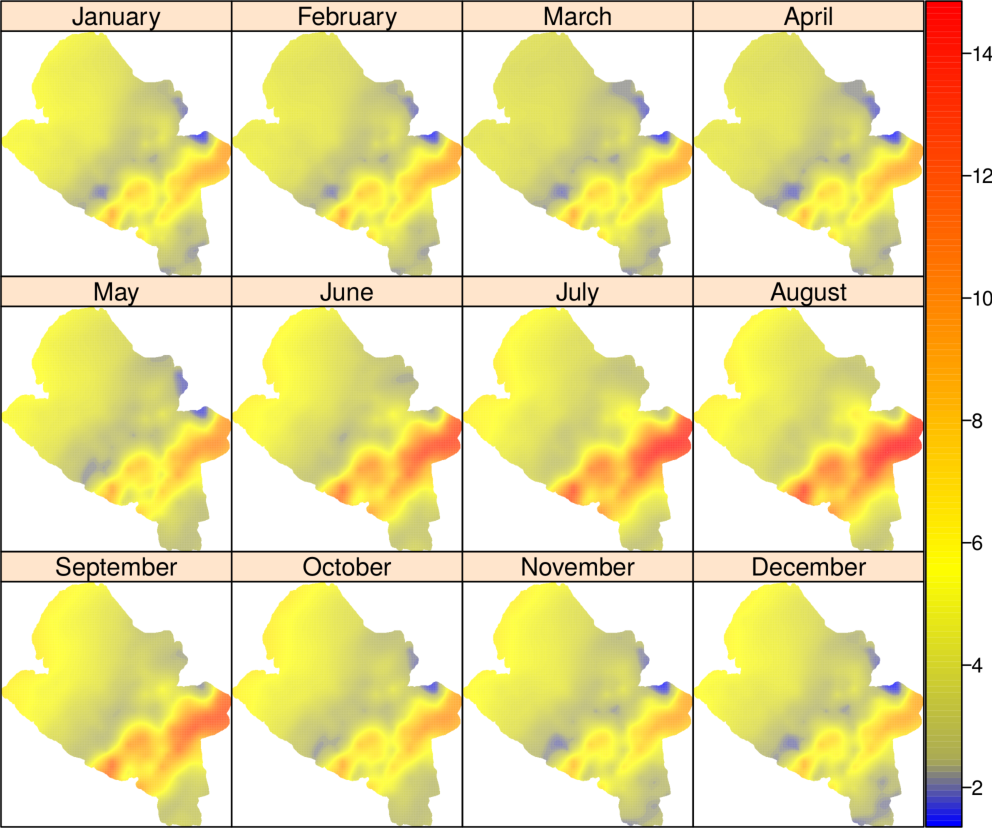
\includegraphics[width = 8cm]{mapMonthsWind.pdf}
  \caption{Velocidad del viento por meses a 50m}
  \label{fig:meses}
\end{figure}

\begin{figure}
  \centering
  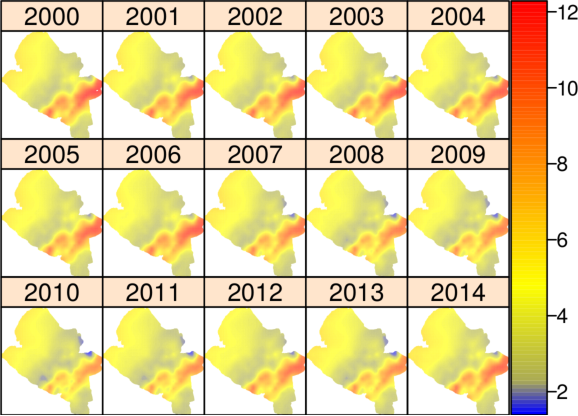
\includegraphics[width = 8cm]{mapYearsWind.pdf}
  \caption{Velocidad del viento por años a 50m}
  \label{fig:anios}
\end{figure}

\begin{figure}
  \centering
  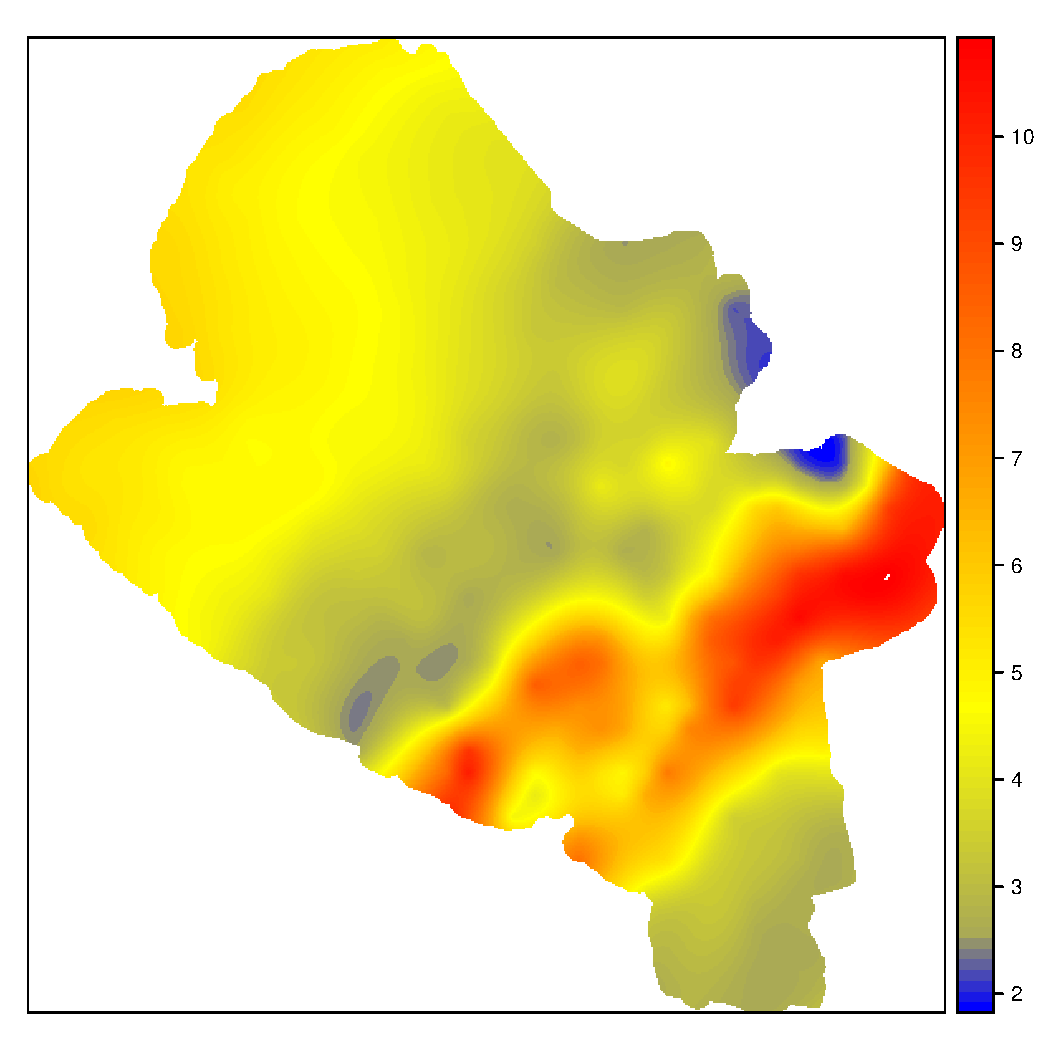
\includegraphics[width = 8cm]{mapGeneralWind.pdf}
  \caption{Velocidad del viento general a 50m}
  \label{fig:total}
\end{figure}



\subsection{Detección de patrones}

Para la detección de patrones se utilizó el algoritmo lcm\_seq propuesto por \cite{uno_lcm_seq},
este algoritmo es una variación de LCM para mineria
LCM\_seq is a variation of LCM for minería de secuencias. 
Este algoritmo encuentra todos los patrones de secuencias que aparecen con frecuencia
en una base de datos dada, cada transacción es considerada una secuencia. El algoritmo sigue el esquema 
llamado lapso de prefijo, pero las estructuras de datos y método de procesamiento se basan en LCM.


Para aplicar este algoritmo se construyo un script el cual convierte los datos de las series de tiempo al
formato de LCM\_seq, para esto se categorizó la dirección del viento en 8 bines, y la velocidad del viento en 13 bines,
como lo muestra la tabla~\reg{table:iddirspeed}, al categorizar según el valor de entrada se concatena el ID de dirección y de velocidad del viento.

\begin{table}
\caption{IDs de velocidad y dirección de viento para cada grupo}
\label{table:iddirspeed}
\centering
\scalebox{0.7}{
\begin{tabular}{c c c c}
\toprule
 ID\_Speed & Speed(m/s)& ID\_Direction & Degree \\
\midrule
1 & 0 - 0.3 & 1 & 337.5 - 22.5 \\
2 & 0.3 - 1.6& 2 & 22.5 - 67.5 \\
3 & 1.6 - 3.4& 3 & 67.5 - 112.5 \\
4 & 3.4 - 5.5& 4 & 112.5 - 157.5 \\
5 & 5.5 - 8.0& 5 & 157.5 - 202.5 \\
6 & 8 - 10.8& 6 & 202.5 - 247.5 \\
7 & 10.8 - 13.9& 7 & 247.5 - 292.5 \\
8 & 13.9 - 17.2& 8 & 292.5 - 337.5\\
9 & 17.2 - 20.8& & \\
10 & 20.8 - 24.4& & \\
11 & 24.4 - 28.5& & \\
12 & 28.5 - 32.7& & \\
13 & 32.7 - inf& & \\
\bottomrule
\end{tabular}}
\end{table}

Los resultados de esta ejecución exigirán una etapa de interpretación y discusión
 de los resultados donde se deberán seleccionar o implementar diferentes
técnicas de visualización. Frecuentemente, al aplicar técnicas de minería de datos
se produce una gran cantidad de resultados donde las técnicas de visualización y
filtrado resultan fundamentales para el la compresión del conocimiento generado.

\subsection{Visualización de patrones}

Para la visualizazión de patrones se tubo en cuenta cuatro atributos de los patrones encontrados, como lo es
la frecuencia, longitud del patrón, diferente velocidad y diferente dirección. Para esta visualización se
construyeron archivos KML(Keyhole markup language) el cual es un lenguaje marcado basado en XML para representar
datos geográficos en tres dimensiones, los KMLs se que se contruyeron fueron con las 50 estaciones de mayor potencial,
en la figura~\ref{fig:speedpattern} se puede mirar el patron que tiene diferentes de velocidades a 50 metros, 
los KML's que se construyeron se los puede descargar del repositorio del
proyecto \footnote{https://github.com/poldrosky/alternar}.

\begin{figure}
  \centering
  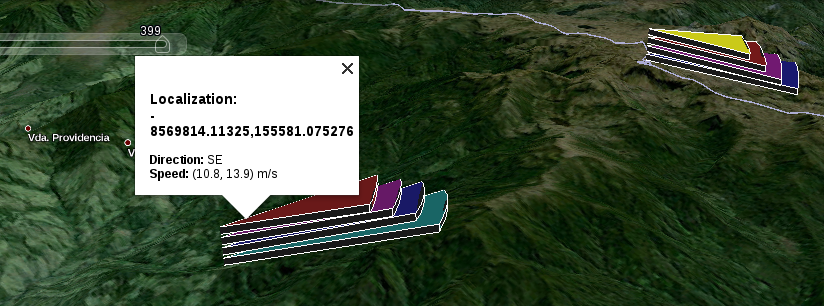
\includegraphics[width = 8cm]{speedpattern.png}
  \caption{Patron con diferentes velocidades a 50 metros}
  \label{fig:speedpattern}
\end{figure}





